\part{Getting started}
\chapter{Installing Tomb Editor}
First of all, you need to download and install the Tomb Editor pack on your computer. It is available eg. \href{https://tombengine.com/}{here}.
\par The default route of Tomb Editor installed is \path{C:\Tomb Editor}. The contents of this main folder are:
\begin{itemize}
    \item Tomb Editor program.
    \item Side programs dedicated to Tomb Editor: SoundTool, TombIDE, WadTool.
    \item Most of the files which are necessary to start a basic project and level for Tomb Engine. (But texture files for room faces must be find somewhere else. But this is still not necessary now, when you start reading this tutorial.)
    \item Other important files for Tomb Editor pack.
\end{itemize}
So when you have the Tomb Editor pack installed on your computer, then you are just ready to start building levels for Tomb Engine. \cite{akyv_tutorial}

\chapter{Starting a new project}
After the installation of Tomb Editor pack, you are ready to make your very first Tomb Engine project. (Level map file extensions are well-known as “PRJ” files, but do not misunderstand: what we call “project” now is not a level, but a whole level set - i.e. your current Tomb Engine game itself, which will be released when you fully made it.)
\par But where do you need to place your projects? Well, NOT in Tomb Editor main folder - that is a place you usually never modify while editing. I suggest placing all of your projects nicely collected in a so-called general project folder. This could be called eg. \path{"My_Tomb_Raider_projects"}, created manually. (I created it in Documents folder.)
\par Each project you make will be placed in its own main folder. Does it mean now you should also create manually a project main folder in the general folder? No, there is a TombIDE wizard which will do the whole project-creating procedure for you.
\par Projects are handled in \textbf{TombIDE (Tomb Integrated Development Environment or TIDE)} program, that is why the whole project-creating procedure is also being done there.
So start \path{TombIDE.exe}, and the panel of TIDE Start page opens up.
Click on “Create a new project” button now.
The first page of a new panel opens up (General Information, \ref{fig:tide1}):
\begin{figure}
    \centering
     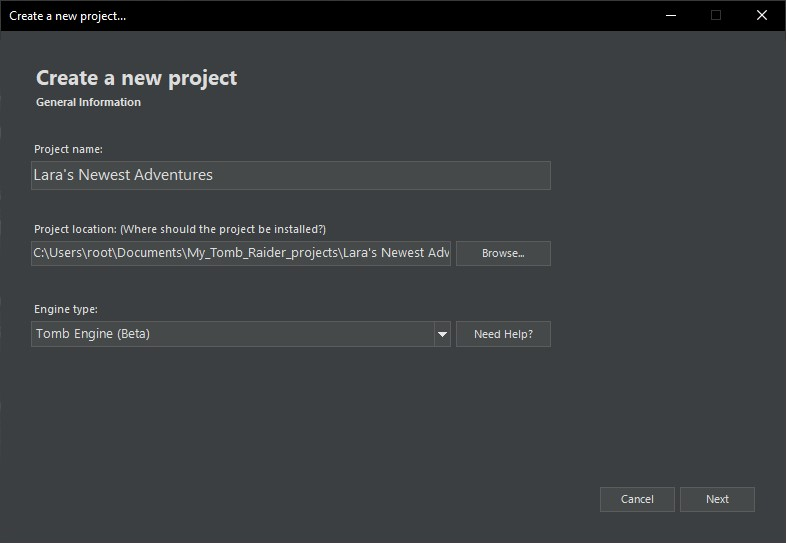
\includegraphics[width=0.75\textwidth]{screenshots/1.jpg}
     \caption{General Information}
     \label{fig:tide1}
\end{figure}

\begin{itemize}
    \item Let's suppose the project you start now has the name of “Lara's Newest Adventures”. So type it now here.
    \item Click on “Browse” button, find and select the general project folder.
    \item After that, the little window in the middle of this first page shows that a subfolder in the general project folder will be created as the main folder of this project, having the project name.
    \item The engine type you choose now is naturally Tomb Engine.
\end{itemize}


\par Now click on “Next” button to continue the procedure on the next page of the panel (Extra Options, \ref{fig:tide2}).

\begin{figure}
    \centering
     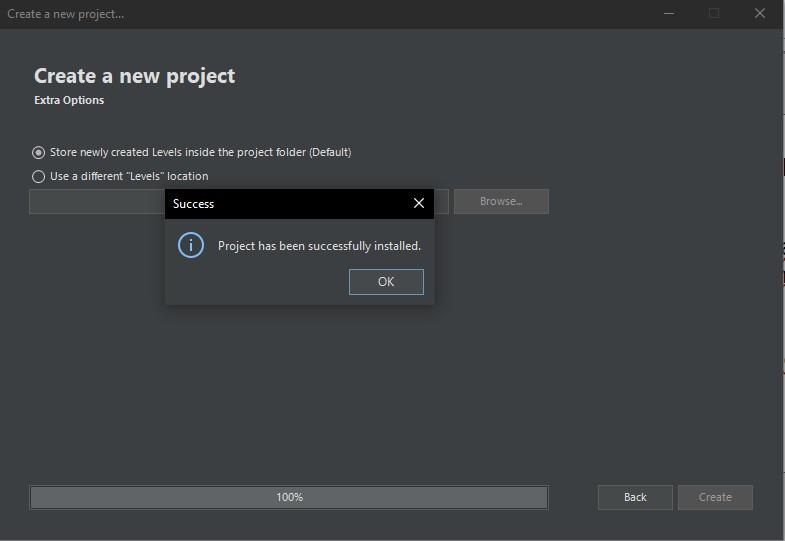
\includegraphics[width=0.75\textwidth]{screenshots/2.jpg}
     \caption{Extra Options}
     \label{fig:tide2}
\end{figure}

\par I suggest changing nothing here. Which means level map files will be handled in a folder called "Levels", which is a subfolder in the main folder of the project. (I mean, this is the default place for level map files, and you, the beginner probably should keep it like this.)
\par Now click on "Create" button here, then look at the increasing bar at the bottom of the panel.
When the bar is at 100 \%, then you get a message that the project has been successfully created (\ref{fig:tide3}).

\begin{figure}
    \centering
     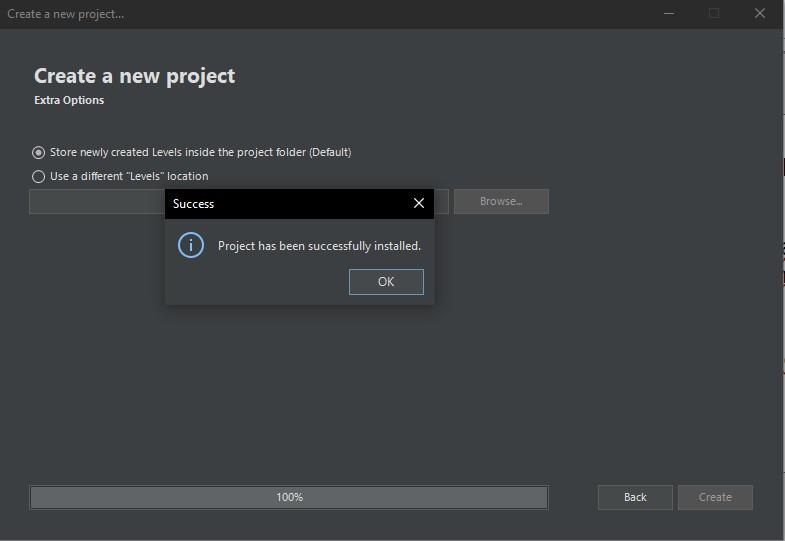
\includegraphics[width=0.75\textwidth]{screenshots/3.jpg}
     \caption{Project has been successfully installed}
     \label{fig:tide3}
\end{figure}

\par And this project main folder has been also created on the selected route, with the basic contents a TEN project should have. (Including Levels folder - still being empty - in that default position., \ref{fig:tide4})

\begin{figure}
    \centering
     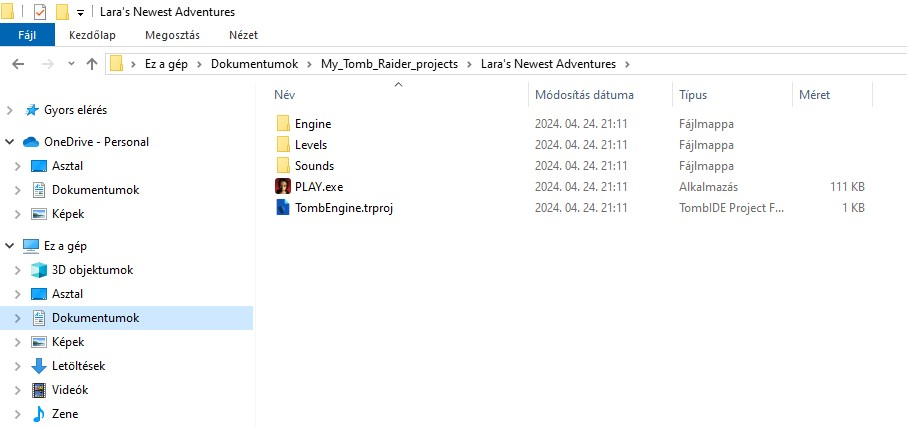
\includegraphics[width=0.75\textwidth]{screenshots/4.jpg}
     \caption{Project directories have been created (Since TEN 1.7., the project main folder has an Assets subfolder as well.)}
     \label{fig:tide4}
\end{figure}

Double-click on that row (or click on "Open selected button" below), so the project opens in TIDE, you will be able to work on it. Each project opened in TIDE has more pages, now you can see its Level Manager page. (See the panel header which names the current project.)
% \par Now click on the red arrow in the upper left corner of the page, to go back to TIDE Start page, closing this project now in TIDE. (Since TEN 1.7., you can see the blue TIDE icon in that corner, instead of the red arrow. If you click on that icon, then a menu opens. One of the menu options is an arrow, with "Back to Start Window..." name. Click on it to go back to TIDE Start page.) \cite{akyv_tutorial} % Referring to old version, changed to fit latest version
\par Now click on the blue TIDE icon in the upper left corner of the page, then a menu opens. One of the menu options is an arrow, with "Back to Start Window..." name. Click on it to close this project now, going back to TIDE Start page.
\cite{akyv_tutorial}

\chapter{What is a level?}
Before we discuss how to start a new level, important to understand, that actually what a "level" is.
\emph{(Don't do anything now, just read and listen.)}
\section{Level map}
Level maps are the editable versions of levels. So when you create, modify a level in the level editor program, then the changes are saved and stored in level map files.
 TE has its own level map formula, whose extension is called \path{PRJ2}.\footnote{Previously level map files was known as files with \path{PRJ} extension.}
 \par At the moment you don't have PRJ2 files, but soon you will create them and save them in Levels folder of the project main folder. (In fact, in subfolders of Levels folder, and each subfolder is dedicated only to one level of the project, having a name which nicely refers to the level name.)
 \section{Playable level}
 The playable version of the level is a level file what the game will play as a level. This playable file is made by a conversion, converted from the PRJ2 level map file of this level. (The conversion will be a very simple task to you: only a simple click on a button.)
 \section{Level script}
Script means game or level data, described simply by typing some texts.
There is a tool in TE pack dedicated to edit script. This is TIDE you have already used to create your project, and you definitely will use it later much to edit your script. \footnote{In TRLE or NGLE there is a "level block" in the script, where all the scripted data of that level are typed. In TE it works the same way - except if the engine for your TE project is TEN. In that case script works a bit differently, as you will see. (Though, a level block also exists there.)}
 \section{Crucial attachments}
 Literally or "only" technically, but levels are useless without their crucial attachments. (Which you will attach in TE to the level map. Then you need to save the map to keep it.)
\begin{itemize}
    \item Item files
    \item Texture files
    \item Sound files and their catalog
\end{itemize}
\subsection{Item files}
An item file (attached to a level) contains all the Moveable and Static objects (Lara, creatures, statues, furniture, effect emitters etc.) and sprites \footnote{In computer graphics, a \textbf{sprite} is a two-dimensional bitmap that is integrated into a larger scene, most often in a 2D video game. \cite{sprite_wikipedia} \index{Sprite}} which can be used in that level.
In TE you can select more than one item file for a level. (And if an object is there in both, then you can set which one of them should be applied in the level.)
\footnote{Unlike the older editors, where only one item file could be selected per level.}
\begin {itemize}
    \item \par Builders using TRLE/NGLE previously definitely know that the extension of an item file is \path{WAD}, acronym standing for \emph{Where's All the Data?} \footnote{WAD is generally a main architectural component of retro games - see e.g. \url{https://en.wikipedia.org/wiki/Doom_modding} for usage in \emph{Doom} custom games.}, made/edited probably with WadMerger program. But it is not obvious any more, if your level editor program is Tomb Editor. In TE WAD extension is usually supported, but not preferred.
    \item \path{WAD2} extension means an enhanced item file (eg. with the feature of UV-mapping \footnote{\textbf{UV mapping} is the 3D modeling process of projecting a 3D model's surface to a 2D image for texture mapping. The letters "U" and "V" denote the axes of the 2D texture because "X", "Y", and "Z" are already used to denote the axes of the 3D object in model space. \cite{UV_mapping_wikipedia} \index{UV mapping}} which is not possible in WAD files). WAD2 files are made and useable only for TE levels, it is the preferred extension here. \\ There is a tool in TE pack dedicated to edit item files, called WadTool. Just open a WAD in it, and save it. It will be saved automatically as a WAD2 item file. (Or you can naturally arrange even a brand new WAD2 in WadTool.)
    \item TEN engine is able to use only specific WAD2 files, which means WAD extension is not supported for TEN engine. (Except if WAD has only objects having non-TEN specific behaviors, like Statics.) \\ You can find a menu option in WadTool, to convert your other item files into a TEN WAD2. \\ "Specific" means eg. TEN Lara object is optimized for TEN, so a "casual" (non-TEN) Lara would not be animated properly there. (Later we discuss it in this tutorial - but not the details, because it is not a TEN WAD2 tutorial.)
\end{itemize}
WAD2 files for a TEN level should be placed in Levels folder, in the subfolder of that level. (It is recommended to use a sub-subfolder there for it.) - Though, technically it is not a must, they can be placed even anywhere in your computer.
\subsection{Texture files}
A texture \footnote{A \emph{texture map} \index{Texture map} refers to a 2D image ("texture") that adds visual detail to a 3D model. The image can be stored as a raster graphic. A texture that stores a specific property—such as bumpiness, reflectivity, or transparency—is also referred to as a \emph{color map} or \emph{roughness map}. \cite{texture_mapping_wikipedia}} file (attached to a level) contains all the texture tiles which can be placed on room faces (floor sector, ceiling sector, wall section) in that level.
\par In TE:
\begin{itemize}
    \item you can select more than one texture file for a level, placing tiles even from each in your level,
    \item not only TGA extension is supported for texture files, but even other ones: BMP, JPG, PNG etc.
\end{itemize}
Texture files for a TEN level should be placed in Levels folder, in the subfolder of that level. (It is recommended to use a sub-subfolder there for it.) - Though, technically it is not a must, they can be placed even anywhere in your computer.
\subsection{Sound files and their catalog files}
Sounds saved in sound files can be emitted mostly by Moveable objects (mostly Lara or other creatures), but even by any effect (like a rumbling earthquake). Etc.
\par Sound files have WAV extensions - just like in the old times.
\par Sound files are not directly attached to a level map, for two reasons:
\begin{itemize}
    \item Sound files for a TEN level should be placed in Sounds subfolder of project main folder. (Though, technically it is not a must, they can be placed even anywhere in your computer.) Initially you can find all the original sounds here of the legacy engines, in their own subfolders. - But naturally you are allowed to edit these contents, modifying, deleting, adding sound files here. \\ These places are needed to be attached to that level.
    \item There must be one catalog file (or, unlike the older editors, even more catalog files), attached to the level, where the sounds you want to attach are named. The main reason is that sounds can have different properties for different levels, and the catalog will describe the properties that this sound will have on this level \\ Sound catalogs can be even older types, familiar from TRLE/NGLE (Sounds.txt or SFX/SAM files of WAD files), or the ones having XML extensions, which are made for TE. Later you will be able to make custom XML files, but some of them are created when saving a WAD2 file. And there are even some preset XML catalogs in Catalogs/TEN Sound Catalogs subfolder of Tomb Editor main folder. \\ There is a tool in TE pack dedicated to edit sound catalogs, called SoundTool. If you want, just open a non-XML catalog into it, and save it as an XML one.
\end{itemize}
\section{Conclusion}
When you start building a new level for your project, then these are your tasks, recommended in this order:
\begin{enumerate}
\item Create a PRJ2 level map file.
\item Add this level to the project.
\item Check the needful contents of the level script. If your script has less contents than that, then the level is useless in the game.
\item Check the main settings (in TE) for the level. If they are wrong, then the level is useless in the game.
\item Check the crucial attachments.
\item You can try to edit something in the level map - then save it.
\item Convert the PRJ2 level map into a TEN playable level.
\item Start the level in the game, try what you have just edited in the map.
\end{enumerate} \cite{akyv_tutorial}

\chapter{Starting a new level map}

\section{Using TombIDE wizard}

\begin{enumerate}
    \item Open the "Lara Newest Adventures" project in TIDE, remaining on Level Manager page.
    \item See the left big window here, with the title of "Level list". As the text says in it, click on it, or - because the text is not available when there is at least one level in this window - click on the "+" button on the upper left corner of the window.
    \item The panel of "Create a New Level" opens (\ref{fig:tide7}):
    \begin{itemize}
        \item \textbf{Level Name}: this level name will be shown in the game for this level. Let's say it is "Test Level 1" now.
        \item \textbf{Use custom PRJ2 / DATA name}: if you tick it, then you can add an alternative name key instead of the default one. \\ Name keys are the names of the most important files of this level. The default name key is mostly the Level Name, except: there cannot be spaces. So eg. for Test Level 1, level files will be auto-created with this name key later: Test\_Level\_1.prj2, Test\_Level\_1.ten etc. \\ Let's suppose we don't want the default name key now, so tick the option and type "Test1" as the name key. (So the file names will be Test1.prj2, Test1.ten etc.)
        \item \textbf{Generate Lua script}: as I said above, there is a scripted part even for TEN. If you untick it, then the wizard will skip this part, not creating the needful contents of the level script. So later you have to create it manually (but before starting the level at the very first time in the game).
        % \\ (The option name is a bit misleading, though, Script.txt and [Level] section are presented in a bit different way for TEN. But it doesn't matter.)%
        \\ Some values in the scripted part you need to define now:
\begin{itemize}
    \item \textbf{Ambient sound ID}: the initial ambient background noise of the level. I suggest accepting this 110.wav now, because later you can change it any time. Or you can click on Open /audio/ button to open Engine \textbackslash Audio subfolder in the project main folder now, to try to find another one. \footnote{Audio subfolder has the original audio file set of The Last Revelation game. Later you can change the contents any time. Now I suggest choosing a WAV above 100 value here, because in that set, background noises are placed on those IDs. However, for TEN you can use any ID for a background noise - but we won't discuss it in this tutorial.}
    \item \textbf{Enable HORIZON (Make the skybox visible in the level)}: the sky above you can be visible in the outdoor areas of the level only if it is ticked. I suggest ticking it, because later you can change it any time. footnote{Skybox and horizon are working together, but they are not the same. But it doesn't matter now.}

\begin{figure}
    \centering
     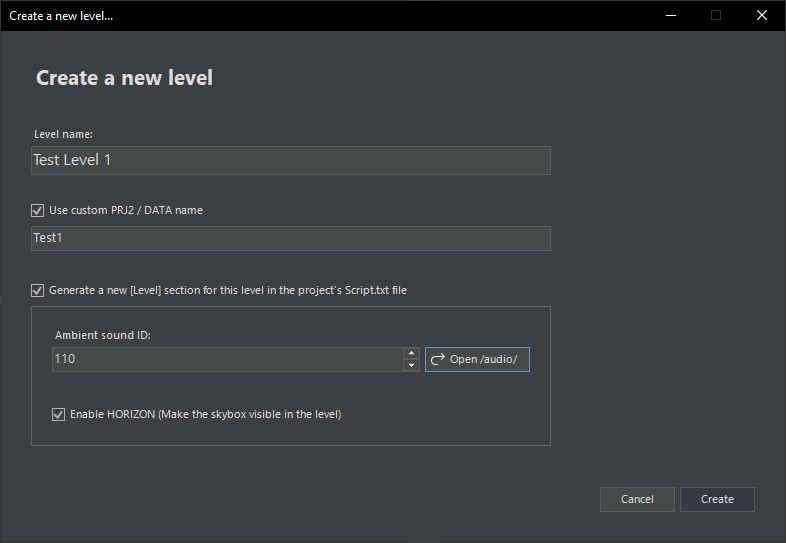
\includegraphics[width=0.75\textwidth]{screenshots/7.jpg}
     \caption{\emph{Create a New Level} panel}
     \label{fig:tide7}
\end{figure}



\end{itemize}
\end{itemize}
\item Click on Create button.
\end{enumerate}

What happened now are:
\begin{itemize}
    \item As I said, each level should have a folder dedicated to it, in Levels folder of this project. Now a dedicated folder to Test Level 1 automatically has been created there, having this level name.
    \item A Test1.prj2 file has been also automatically created, in Test Level 1 folder.
    \item The main settings of this level have also been done properly.
    \item Some crucial attachments of the level has been automatically attached. (Later we discuss it in the tutorial.)
    \item In Level list window of this project (on Level Manager TIDE page), a row for this level has been also automatically created (\ref{fig:tide8}).
    
\begin{figure}
    \centering
     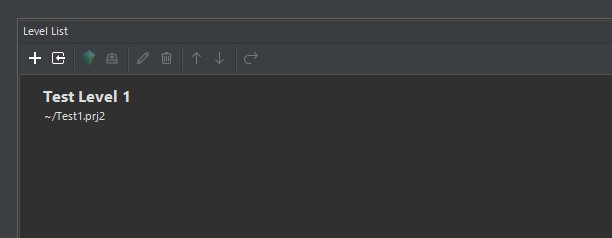
\includegraphics[width=0.75\textwidth]{screenshots/8.jpg}
     \caption{\emph{Level list} panel showing level you've created}
     \label{fig:tide8}
\end{figure}

    \item The needful contents of the level script has been also automatically created. (Later we discuss it in the tutorial.)

\end{itemize}
Now you can click on the arrow menu option in the menu of the blue TIDE icon to go back to the Start page of TIDE.
%\\ But TIDE now asks you if you want to save what you have just did. Naturally accept it. \\ (However, operations you did in TIDE are automatically saved. Except if those are rows typed in the script.) % It was not asked to save by the application during testing of this tutorial...

